\section*{Реализация и анализ МЭД}
\addcontentsline{toc}{section}{Реализация и анализ МЭД}
\subsection*{Моделирование валютного курса}
\addcontentsline{toc}{subsection}{Моделирование валютного курса}

\textbf{Задание:}\\
Приказать изменение валютного курса и его зависимость от параметров, провести анализ модели.\\

\textbf{Решение:}\\
Валютный курс является одним из основных экономических показателей, он оказывает влияние на международную торговлю, инвестиционные потоки, валютно-обменные операции, международные конкурентные преимущества стран и блоков и другие составляющие мировой экономики.\\

Задача определения равновесного курса рубля представляет большое значения для эффективного управления народным хозяйством. Особую значимость определение равновесного курса приобретает для основных мировых валют, образующих фундамент мировой экономики и мировой валютной системы.\\

Результаты моделирования позволяют теоретически обосновать некоторые важные тенденции, наблюдаемые в мировой экономике.\\

Пусть $e_i$ -- валютный курс, $D_i$ -- сумма в иностранной валюте, $R_i$ -- сумма в национальной валюте $i$-й сделки. Между собой данные параметры связаны следующим образом:

\[e_i D_i = R_i\]

В связи с тем, что большинство международных сделок на российском рынке происходит в долларах США, то в качестве иностранной валюты в модели будет рассматриваться только доллар США.\\

Валютный курс можно определить как усредненное взвешенное значение по всем сделкам ($N$ сделок), то есть:

\[e = \sum_{i=1}^N \dfrac{D_i}{\sum_{i=1}^N D_i} e_i = \sum_{i=1}^N \dfrac{D_i}{\sum_{i=1}^N D_i} \dfrac{R_i}{D_i} = \dfrac{\sum_{i=1}^N R_i}{\sum_{i=1}^N D_i} \]

Таким образом, валютный курс равен совокупной сумме средств в отечественной валюте, делённой на совокупную сумму средств в иностранной валюте, обращающихся на валютном рынке, и итоговый результат можно представить как:

\[e = \dfrac{\sum R^{CA} + \sum R^K + \sum R^{CB}}{\sum D^{CA} + \sum D^K + \sum D^{CB}} \]

где $R^{CA}, D^{CA}$ -- средства в отечественной и иностранной валюте соответственно, происходящие по счёт текущих операций; $R^{K}, D^{K}$ -- средства в отечественной и иностранной валюте соответственно, происходящие по счёту движения капитала; $R^{CB}, D^{CB}$ -- средства в отечественной и иностранной валюте соответственно, происходящие по счёту изменения официальных валютных резервов ЦБ.\\

В рассматриваемой модели имеется допущение о том, что модели на уровне баланса текущих операций, включают равноправные двусторонние отношения двух стран-контрагентов и совместные действия монетарных органов по поддержанию стабильности валютного курса на желаемом уровне.\\

Модель удовлетворяет следующим утверждениям:
\begin{enumerate}[topsep=0pt,itemsep=-1ex,partopsep=1ex,parsep=1ex]
	\item Мир модели представлен двумя равноправными странами. Экспортные потоки одной станы представляют импорт партнёра симметрично по отношению друг к другу: $I^* = E$, $E^* = I$.
	\item ЦБ осуществляют жёсткое регулирование движения капитала либо законодательными мерами, либо полностью удовлетворяя спрос на валюту путём продажи за счёт изменения валютных резервов, то есть на данном этапе учитываются только текущие операции и движение капитала.
	\item Счёт текущих операций состоит из операций экспорта – импорта, учитывая счёт услуг, и не учитывает счета односторонних трансфертов.\\
\end{enumerate}

Тогда получается:

\[ \sum R_i^{CA} = I \sum D_i^{CA} = E\]

где $I$ -- спрос в национальной валюте на иностранную со стороны импорта; $E$ -- предложение иностранной валюты со стороны экспорта.\\

\newpage

Пусть $\sum R_i^K = K^-$, $\sum D_i^K = K^+$ -- оответственно сумма средств оттока (спроса в национальной валюте на иностранную) и притока (предложения иностранной валюты) по счёту движения капитала. Тогда исходная формула преобразуется следующим образом:

\[ e_t = \dfrac{I_t + K^-}{E_t + K^+} \]

где симметрично определены валютные курсы вовлечённых в рассмотрение стран.\\

В данной модели $E_t$ -- объём экспорта, который напрямую зависит от реальных условий торговли, то есть может быть представлен следующим образом:

\[ E_t = P_t^* k_E \sqrt[3]{(Q_{t-1}^2 Q_t)} e^R_{t-1} \]

где $k_E \sqrt[3]{(Q_{t-1}^2 Q_t)}$ отражает то, что экспорт является частью совокупного выпуска; $Q_t$ -- совокупный реальный выпуск (например, реальный ВВП); $P^*_t$ -- совокупный уровень цен партнёра; $t, t-1$ -- начало и конец периода соответственно; $e^R_{t-1} = e_{t-1} \dfrac{P^*_{t-1}}{P_{t-1}}$ -- величина реального валютного курса.\\

\[ I_t = E^*_t = P_t k_I \sqrt[3]{(Q_{t-1}^{*2} Q_t^*)} e^{R}_{t-1} \]

где $P_t$ -- совокупный уровень цен, $Q^*_t$ -- совокупный реальный выпуск партнёра.

\[ K^+ = k_{K^+} P^*_t \sqrt[3]{(Q_{t-1}^{2} Q_t)^\theta} e^{R}_{t-1} \]
\[ K^- = k_{K^-} P^*_t \sqrt[3]{(Q_{t-1}^{*2} Q_t^*)^\rho} e^{*R}_{t-1} \]

где $e^{*R}_{t-1} = \dfrac{1}{e^{R}_{t-1}}$.

\[ e_t = \dfrac{I_t + K^-}{E_t + K^+} = \dfrac{P_t k_I \sqrt[3]{(Q_{t-1}^{*2} Q_t^*)} e^{R}_{t-1} + k_{K^-} P^*_t \sqrt[3]{(Q_{t-1}^{*2} Q_t^*)^\rho} e^{*R}_{t-1}}{P_t^* k_E \sqrt[3]{(Q_{t-1}^2 Q_t)} e^R_{t-1} + k_{K^+} P^*_t \sqrt[3]{(Q_{t-1}^{2} Q_t)^\theta} e^{R}_{t-1}}  = \]

\[ = \dfrac{P_t \sqrt[3]{(Q_{t-1}^{*2} Q_t^*)^\rho} \left(k_I \sqrt[3]{(Q_{t-1}^{*2} Q_t^*)^{1 - \rho}} + k_{K^-} \right)}{P_t^* e^2_{t-1}\left( \dfrac{P^*_{t-1}}{P_{t-1}} \right) \sqrt[3]{(Q_{t-1}^{2} Q_t)^\theta} \left( k_E \sqrt[3]{(Q_{t-1}^{2} Q_t)^{1-\theta}} + k_{K^+} \right) } \]

\newpage

где $\theta > 0$, $\rho > 0$.

То есть $\dfrac{k_I \sqrt[3]{(Q_{t-1}^{*2} Q_t^*)^{1 - \rho}} + k_{K^-}}{k_E \sqrt[3]{(Q_{t-1}^{2} Q_t)^{1-\theta}} + k_{K^+}} = (k')^3 = const$, тогда:

\[e_t (e_{t-1})^2 = \dfrac{k' P_t}{P^*_t} \dfrac{Q_t^{*\frac{\rho}{3}}}{Q_t^{\frac{\theta}{3}}} \left( \dfrac{k' P_t}{P^*_t} \dfrac{Q_t^{*\frac{\rho}{3}}}{Q_t^{\frac{\theta}{3}}} \right)^2 \]

Следовательно:

\[ e_t = \dfrac{k' P_t}{P^*_t} \dfrac{Q_t^{*\frac{\rho}{3}}}{Q_t^{\frac{\theta}{3}}} \]

В данной модели переменные $P$, $P^*$ -- уровни цен и $Q$, $Q^*$ -- совокупные продукты, являются экзогенными переменными. Другими важнейшими детерминантами поведения валютного курса являются показатели движения капитала между странами, определённые величинами $\rho$, $\theta$.\\

Коэффициент $k'$ является курсом рубля к доллару США начальной точки периода модели. $\theta$, $\rho$ -- настраиваемые параметры. В качестве рассматриваемого периода возьмем период с 2013 по 2019 года. $P_t$ -- совокупный уровень цен за литр газа в России (в долларах США), $P_t^*$ -- совокупный уровень цен за литр газа в США (в долларах США),  $Q_t^*$ -- реальный ВВП США (в долларах США); $Q_t$ -- реальный ВВП России (в долларах США).\\

Данные для расчётов были взяты с сайта Мирового банка, с сайта Центрального банка и сайта U.S. Energy Information Administration.\\

При параметрах $\theta = 3.19$, $\rho = 2.995$ получили следующий результат. (Рисунок \ref{fig:currency1})
\begin{figure}[h]
	\centering 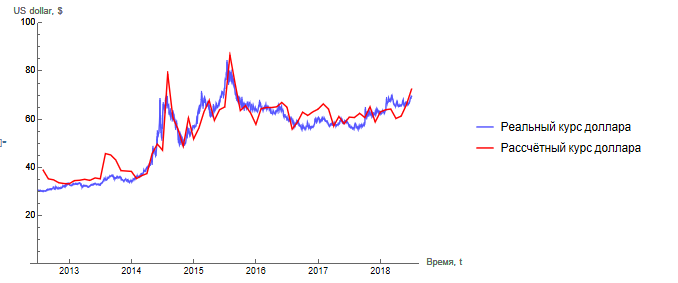
\includegraphics[scale=0.55]{currency1}
	\caption{Результаты моделирования}
	\label{fig:currency1}
\end{figure}

\newpage

Исходя из полученного графика можно сделать вывод о том, что модель достаточно четко показывает изменение тенденции валютного курса, однако предсказанные ей значения не всегда являются точными. Модель показывает хорошие результаты в долгосрочной перспективе и может быть использована для долгосрочного или среднесрочного моделирования.